\section{Architecture \& Design}
\label{sec:architecture_design}

\paragraph{Primary textual contributors.}
\mbox{}\\\emph{Thomas Kretschmann}

This chapter presents the architecture and the related design of SWTcamper. First, we show which architectural model we have chosen and justify our decision. Then we will explain the implementation based on this and how individual design decisions can be derived from it. In particular, we will go into the design of the database schema and the representation of each entity. Finally, the design patterns and design principles used are presented and briefly explained.

\subsection{Choice of Architecture}
For the architecture of SWTcamper, we opted for the \textit{Model-View-Controller} architecture pattern, as this encapsulates the frontend from the backend and allows the graphical user interface to be changed while the backend remains the same. This is particularly interesting in view of the fact that future SWL students should provide the application with a web front end. \\
In contrast, the application we built runs completely locally, although one could imagine offering the database or the \textit{Docker container} that contains it on a remote machine. \\
Due to the clear division of the layers belonging to the MVC pattern (easily recognizable in fig. \ref{fig:architecture}), it was also possible to clearly distribute associated tasks to team members with ease.

\begin{figure}[h]
	\centering
	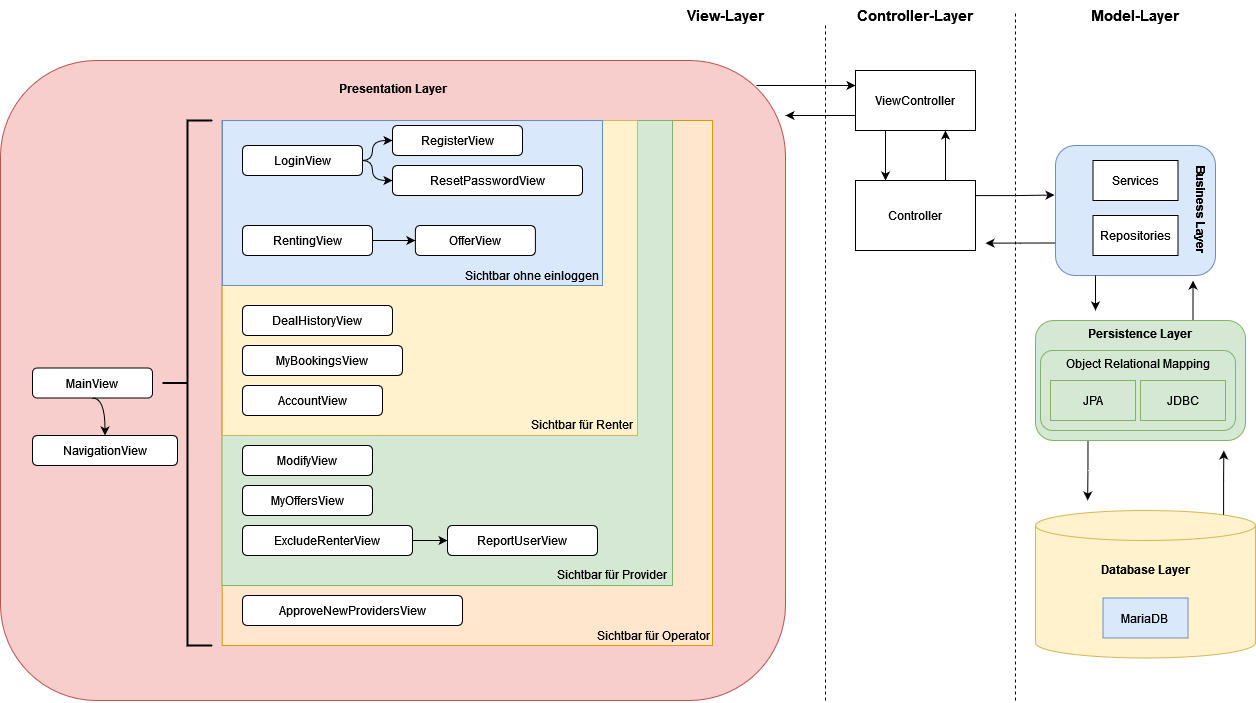
\includegraphics[width=15cm]{resources/images/architecture.drawio.png}
	\caption{General Architecture of SWTcamper}
	\label{fig:architecture}
\end{figure}

\subsubsection{Layered MVC in general}
The Model-View-Controller pattern is an architecture or design pattern that offers flexible program design, makes it easier to change or expand it later, and allows the individual components to be reused.
Applications designed according to the principles of MVC consist of three interchangeable components:

\begin{itemize}
	\item \textbf{The model} consists of several model classes. Each represents a basic entity within the data structure used. They also provide basic data operations that are not necessarily part of the basic program logic. This includes, for example, the individual entities on the basis of which the application runs, or the services that provide the necessary values from the database and can already process them to the necessary degree.
	
	\item \textbf{View} classes provide the graphical user interface. The model classes provide the displayed data, but there is no direct connection between the two program parts. The controller informs the components of the surface display about changes to the model and they adjust the displayed content if necessary.
	
	\item \textbf{The controller} classes act as a connector between view and model components. The view forwards user actions to the controller, which executes the underlying program logic. If necessary, the logic informs individual views about changes to the model in order to enable an appropriate reaction to them.
\end{itemize}

\subsubsection{JavaFX (view)}
JavaFX is an open source framework used to create graphical user interfaces (GUI). In SWTcamper we used the JavaFX feature that allows to fully define the view part in FXML files. The views were only generated programmatically for dynamic program parts, like the list of available displays or the operator dashboard. The view is then created at runtime of the program using the FXML files and JavaFX. The view controllers are the controllers of the individual views, which not only take care of event handling, but also request and forward data from the 'real' controllers.

\subsubsection{Spring boot (view, controller, model)}
Spring Boot is an open source framework that offers many functionalities for developing a standalone application. It simplifies the software development process by reducing complexity and providing a clear structure. In our case, it is used in every layer of the MVC pattern. \\
In order for the framework to know how to deal with each class, there are annotations that allow Spring Boot to create the necessary environment for the classes. An example of this is the \textit{@Service} annotation, which is placed above each of our service classes, or \textit{@Component}, which is used above each controller. \\
Simply using Spring Boot doesn't guarantee quality, but it does provide a structure that makes it easier to develop quality software and avoid mistakes.

\subsubsection{JPA (model)}
Combined with Spring Boot, the \textit{Java Persistence API} allows us to convert Java objects to
Database objects and vice versa. Various settings can be made through annotations in the entity classes in order to implement the desired database schema automatically.

\subsubsection{Docker (model)}
Docker is open source software that allows us to run applications in a virtual container environment. Many software vendors already provide preconfigured images that allow their application to run in a containerized Docker environment. We used Docker to run our \textit{MariaDB} database in it.

\subsubsection{MariaDB (model)}
MariaDB is an open-source relational database. We use it to store our data consistently. MariaDB also offers its own Docker image, making it a good choice for our application.

\subsection{Design Implementation}
In order to understand which components we need for the application and how best to proceed, we created a use case diagram (fig. \ref{fig:use-case-diagram}) and an ER diagram (fig. \ref{fig:er-diagram}) which have changed over the course of the project.

\begin{figure}[h]
	\centering
	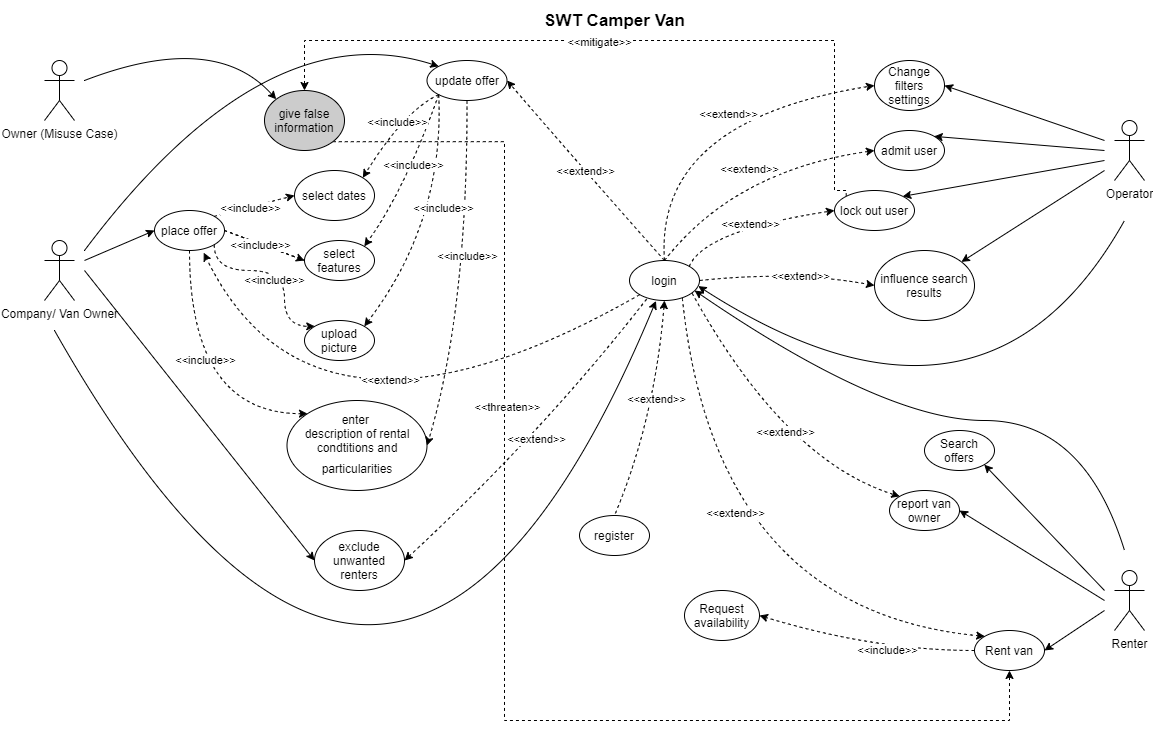
\includegraphics[width=12cm]{resources/images/use-case-diagram.png}
	\caption{Use Case Diagram}
	\label{fig:use-case-diagram}
\end{figure}

\paragraph{Basic Structure}
The heart of SWTcamper is the \textit{MainView} and its associated view controller, which is called directly from \textit{App.java} (starting point for JavaFX applications) when the program starts. Via imports, it contains all other FXML views that are added or removed via the controller depending on the \textit{NavigationViewController}. (trying to show in fig. \ref{fig:architecture}) When the program starts, the \textit{RentingView} is loaded first via the \textit{changeView()} method, which contains all available displays. To do this, the \textit{AnchorPane} 'mainStage' in the \textit{MainView} is first completely emptied and then filled with the \textit{RentingView} mentioned. If the user now presses a button in the \textit{NavigationView} (buttons are displayed depending on the \textit{UserRole} (also taken from fig. \ref{fig:architecture})), the \textit{MainViewController} is instructed via its view controller to repeat the same procedure for the newly selected view. In order to differentiate between the views, a suitable string must be passed to the \textit{changeView()} method (e.g. 'home' for the \textit{RentingView} or 'history' for the \textit{DealHistoryView}). Since all view controllers are already initialized when the program starts, all other view controllers must also be imported into the \textit{MainViewController} so that a reload method can be called for each one individually.

\subsection{Class diagrams}
We made a class diagram in the first sprints. Since our classes have changed since then, we wanted to include an automatically generated class diagram at this point; However, since this is much too big, we tried to split it up into its most important classes and integrate them separately. The diagrams can be viewed in the Additional Material (fig. \ref{fig:cd:controller-services} and fig. \ref{fig:cd:entities}).

\subsection{Data model \& Design decisions}
In order to get an overview of the entities to be implemented and how they interact, we created an ER diagram at the beginning of Sprint 0 (fig. \ref{fig:er-diagram_draft}), which only changed slightly over the course of the project has (figure \ref{fig:er-diagram}). In this chapter we present our entities and their structures.

\paragraph{Booking}
The Booking class is required to bind a user to an ad. To do this, it has an ID that is automatically generated by the database (through the \textit{@Id} and \textit{@GeneratedValue} annotations), a user who wants to rent the associated ad, the ad itself, a start date and an end date. Furthermore, there are the two boolean fields \textit{active} and \textit{rejected}. A booking is created with \textit{active = false} and remains inactive until accepted; if it is rejected, the field \textit{rejected}, which was also created with \textit{false}, is set to \textit{true}. The combination of these two values is used at several points in the application to determine states:

\begin{table}[h]
	\centering
    \caption{\label{tab:booking-variables}Deriving logic from combination of variables in Booking class}

	\begin{tabular}{|c|c|c|c|}
		\hline
		&  & \multicolumn{2}{c|}{active} \\
		\hline
		&  & true & false \\
		\hline
		rejected & true & \begin{tabular}[c]{@{}c@{}}Offer ended early,\\gets listed in offer history\end{tabular} & / \\
		\hline
		& false & \begin{tabular}[c]{@{}c@{}}Offer can not get modified\\or deleted\end{tabular} & \begin{tabular}[c]{@{}c@{}}Provider sees offer as\\``New request for offer''\\(not yet in offer history)\end{tabular} \\
		\hline
	\end{tabular}
\end{table}

\paragraph{Filter}
The Filter class is the only entity class in SWTcamper that is not stored in the database. It contains all the fields from \textit{Offer} and \textit{Vehicle} that are required for a good search. When the search is started, a new filter instance is created and the necessary fields are set. This instance is then passed to the \textit{OfferController}, which uses it to filter the list of all ads and returns a new list of ads that match the filter instance.

\paragraph{LoggingMessage}
Logging messages are generated by almost all services and are required to be able to track events. A list of logging messages can be viewed as an operator via the \textit{AccountView} and downloaded as a log file. Since all logging messages that occur are also stored in the database, each has a unique and automatically generated ID and a time stamp for which it was created. The enum \textit{loggingLevel} indicates how important the logging message is (INFO, WARNING, ERROR) and there is also a message so that the viewer knows what it is about.

\paragraph{Offer}
The offer class was implemented first in SWTcamper together with the vehicle class. In the course of development, however, it was expanded and improved. It is needed to display offers - one of the basics of SWTcamper. Objects of this class have an ID automatically generated by the database, a user who created the offer, title, pick-up location, contact details via which the creator would like to be reached, special features of the offer (such as things that are not already covered by SWTcamper ) and a price. Via \textit{active} the creator can specify whether the offer should be publicly listed and if \textit{promoted} is \textit{true} the offer will be highlighted in the list; this function can only be changed by operators, but is visible to all users. Of course, each offer also contains a permanently associated vehicle object with all its values and lists for blocked dates for which the offer cannot be booked, non-overlapping bookings and rentalConditions, with which the creator specifies conditions to which the renter adheres has to hold. \\
The \textit{offeredObjectType} field is no longer used in our version of SWTcamper; however, it would be possible to extend the application here.

\paragraph{Picture}
Originally it was planned that the images stored in SWTcamper for the vehicles would be completely loaded into the database; however, there were many problems finding the right data type and there were many errors that the database could not store objects of this size. So next we switched to storing a list of paths in the Vehicle object. However, this list was also too long for the database from around three images onwards. \\
As a solution, we have therefore created our own repository for the images. In addition to the obligatory ID, each entry contains the path to the image and the ID of the vehicle to which it is to be assigned. \\
Unfortunately, this approach means that images can only be stored locally and do not work in a distributed system. However, since our application only had the requirement to run locally anyway, that was fine for this framework.

\paragraph{User}
In addition to an automatically generated ID, the User class also has attributes for the username, first and last name, email address, telephone number and password. The \textit{userRole} attribute indicates which role the user assumes when using the application and which authorizations he has as a result (cf. view illustration in fig. \ref{fig:architecture}). Related to this there is also the attribute \textit{enabled}, which is only set to \textit{false} when a user registers as a new provider, since it was a requirement that these people should first be checked before they can create new offers. As long as a user has the role of provider and \textit{enabled} is set to \textit{false}, he has the same powers and options as the \textit{userRole} Renter. \\
Another boolean field is \textit{locked}, which is required to globally block a user; its application options are therefore severely limited. In contrast to this possibility, which can only be carried out by an operator, there is also one for providers with which other users can be excluded from their offers. To do this, User objects use a list \textit{excludedRenters}, in which the IDs of the users to be excluded are stored.

\paragraph{UserReport}
UserReports are required so that one user (as of UserRole Provider) can report another. A submitted UserReport is then stored in the database (again has an automatically generated ID) and has an \textit{active} boolean field set to \textit{true} until the report is processed (\textit{accepted} or \textit{rejected}) by an operator. In order to make it easier for the decisive operator to make his decision, each UserReport contains both the username of the reporter and the reported person and a message explaining why the reporter submitted the report.

\paragraph{Vehicle}
Just like the offer class, the class for the vehicles themselves plays a very central role, which is why it was implemented first. It contains very rudimentary attributes to represent the vehicles offered; in addition to the automatically generated ID, this includes the brand, model, year of construction, length, width and height, the type of connection, the number of seats and the number of beds. Simple boolean variables were used to describe whether the vehicle has a roof tent, roof rack, bike rack, shower, toilet, kitchen unit or refrigerator. There are also separate enumerations for the type of vehicle and the type of fuel.

\subsection{Design Principles}

\subsubsection{General Principles}

\paragraph{Hide information}
Similar to what is explained in SOLID's Open-Closed-Principle (\ref{subsec:solid:ocp}), we have applied the 'public' and 'private' access modifiers as far as possible, so that the classes are encapsulated as much as possible. However, we really only used 'public' and 'private' and neglected e.g. 'protected', which only allows visibility within the current package. Implementing this would improve the quality of the software and could well be done in another sprint.

\paragraph{Loose Coupling}
The parts of SWTcamper's Model-, View- and Controller components are clearly seperated from each other and communicate only through interfaces.

\paragraph{Program to an interface, not an implementation}
In SWTcamper we have interfaces for our repositories for the database, for our backend controllers and for our entities. Since we didn't apply this principle from the beginning, but relatively late, we didn't build the interfaces for the entities into the rest of the code, so that they are instantiated directly and not via their interfaces (which would need casts to normal classes anyway). This task would be a good fit for another sprint and shouldn't take much time. In the meantime, the interfaces still represent a kind of 'security template'. For the first two class groups, however, we have applied it according to the principle.

\paragraph{High Cohesion}
This is pretty similar to SOLID's SRP (\ref{subsec:solid:srp}); as mentioned there our classes mostly have only one purpose. Improvments could be made in the MainViewController which also includes the database scanner.

\paragraph{Encapsulate Logic}
This principle was implemented in our application primarily by the fact that the frontend controllers do not have direct access to the backend controllers, but only to the methods from the backend controllers' interfaces.

\subsubsection{SOLID Design Principles}

\paragraph{Single-Responsibility-Principle}
\label{subsec:solid:srp}
For SWTcamper we implemented contract classes and DTO objects. Through this
feature we are able to display the objects of the database with additional information that
can be useful to the user without modifying the objects themselves. Real changes to the objects
are only carried out by saving, deleting or updating operations to ensure that we comply with them
the principle of individual responsibility. \\
Otherwise, our classes mostly have only one purpose. An exception is the MainViewController, which, in addition to managing the other view controllers, also scans the database for changes every second.

\paragraph{Open-Closed-Principle}
\label{subsec:solid:ocp}
By using the MVC pattern it is possible to exchange the frontend without changing the backend. Replacing the database with another one wouldn't be difficult either, as long as JPA is still able to map the objects correctly. This is made even easier by the fact that our database is made available in a container using Docker, which is easier to exchange than without. \\
Furthermore, it would be possible to extend our existing interfaces; however, this was not explicitly valued during development. Instead, we have kept as much internals as possible private, so that classes are encapsulated from the outside as much as possible, which has worked almost completely with a few exceptions.

\paragraph{Liskov's Substitution-, Interface-Segregation- and Dependency-Inversion Principles}
Since we did not go into design principles too much when planning, we did not find any examples for these principles in our application. It is possible that SWTcamper is less suitable for this in its current form. \\
A possible implementation of Liskov's substitution principle would be to implement the IUser interface in the three different user classes Renter, Provider and Operator, instead of implementing it via an enumeration of UserRoles as we did. That would certainly be a point that could be improved in future sprints.

\subsection{Design Patterns}

\subsubsection{Behavioral patterns}

\paragraph{Observer Pattern}
\label{subsec:observer-pattern}
We would have liked to have used this pattern to implement the notifications in such a way that the database automatically sends notifications to all observers (push notification). Unfortunately, we found that MariaDB does not support such functionality. But it was possible to implement a so-called entity listener via Spring Boot annotations; This caused a thread to be started in the background, which checked for changes to the respective entity objects at regular intervals and executed the desired functionality if there was a change. However, inconveniently, in our application this caused the notification dots (the objects that the thread should change when an entity changes) to flicker in the navigation bar, so we decided to implement such a scanner ourselves, which actually worked better: \\
To do this, we implemented the \textit{listenForDataBaseChanges()} method in the \textit{MainViewController}, which fetches the necessary objects from the database and saves them in local variables. After the next fetch, it then compares these variables with the new data and executes the corresponding functionalities if the two data sets are different differentiate. So that this is possible at regular intervals, the method was provided with \textit{@Scheduled(fixedDelay = 1000)}, which also starts a new thread in which, in contrast to the first implementation, the time intervals can be controlled. This implementation also corresponds to the pull notification of the observer pattern.

Furthermore, we used properties in many places in the application and either bound them to others or set EventListeners on them so that dependencies adjust automatically without having to trigger the functionality separately. \\
The (forced by JavaFX) use of observable lists is also to be assigned to the observer pattern, since changes in the lists automatically cause a change in the objects in which they are used.

\subsubsection{Creational patterns}

\paragraph{Singleton Pattern}
Since the structure of SWTcamper is designed in such a way that the \textit{MainView} holds all other views (cf. fig. \ref{fig:architecture}), only one object is created at the start of the \textit{MainViewController} and the \textit{NavigationViewController}, which are permanently displayed and their contents are only change. However, both are also referenced in other view controllers using Spring Boot's \textit{@Autowired}, so at this point we are not 100 percent sure how the framework handles these classes exactly. \\
It would also have been nice to have the database scanner explained in section \ref{subsec:observer-pattern} in its own class, so that it would only be instantiated once - independent of the \textit{MainViewController}. However, it can be assumed that this will only happen once.

\paragraph{Factory Method}
We didn't use this method explicitly, but because we use the Spring Framework and provide many similar classes with the same annotations (\textit{@Component}, \textit{@Service}, \textit{@Entity}, \textit{@Repository}), they use the same interfaces and therefore also have the same standard methods , such as \textit{initialize()}. \\
An explicit implementation might be possible with the ViewControllers; Due to the component-based structure of the application, however, our classes differ so much that sharing interfaces is of little use.

\subsubsection{Structural patterns}

\paragraph{Decorator Pattern}
Initially, to create a new ad and to edit an ad, we had two different views and controllers. However, since the two functionalities are so similar, we have combined them in a view (and thus a controller) \textit{ModifyView}. There is a boolean variable to distinguish between creating a new ad or editing an existing one. The decorator pattern could have been used here, which would extend the class with additional functionality at runtime. However, it is questionable whether this would bring a real advantage given the size of our application and the class.

\paragraph{Pipes and Filters}
We used functional programming in SWTcamper in several places, especially when processing lists (e.g. for filters), and lined up the methods so that the output of the last processing step was always the input for the next.

\subsection{Summary}
In SWTcamper we have applied many of the design principles we are familiar with - partly consciously and partly unconsciously. In some cases, we only implemented them when writing this report, after hearing from them again. Overall, we could definitely implement more with more time and also with higher accuracy. In addition, it would also be good in the future to go into the principles more at the beginning of the architecture and not only later on, but in retrospect we neglected that a bit too much.